% ===================================================================
%  Week 6 — Frequency Domain (Fourier)
% ===================================================================
\documentclass[10pt,aspectratio=169]{beamer}
% ===================================================================
%  Shared Beamer preamble for "Practical Image Processing"
%  English slides. Compile with pdfLaTeX.
% ===================================================================

\usetheme{metropolis}
\usepackage[T1]{fontenc}
\usepackage[utf8]{inputenc}
\usepackage{lmodern}
\usepackage{listings}
\usepackage{tcolorbox}
\usepackage{fontawesome5}
\usepackage{booktabs}
\usepackage{amsmath,amssymb}
\usepackage{tikz}
\usepackage{pgfplots}
\pgfplotsset{compat=1.17}
\usetikzlibrary{arrows.meta,positioning,shapes.geometric,fit,backgrounds,matrix}
\tcbuselibrary{skins,breakable}

% ---- Palette --------------------------------------------------------
\definecolor{coursePrimary}{HTML}{1B4965}   % deep blue
\definecolor{courseAccent}{HTML}{E76F51}    % coral
\definecolor{courseGood}{HTML}{2A9D8F}      % teal
\definecolor{courseBad}{HTML}{C0392B}       % red
\definecolor{courseInfo}{HTML}{2980B9}      % blue
\definecolor{codeBg}{HTML}{F5F6FA}
\definecolor{codeKw}{HTML}{8E44AD}
\definecolor{codeStr}{HTML}{2A9D8F}
\definecolor{codeCom}{HTML}{7F8C8D}

\setbeamercolor{frametitle}{bg=coursePrimary}
\setbeamercolor{progress bar}{fg=courseAccent}
\setbeamercolor{alerted text}{fg=courseAccent}
\metroset{block=fill,sectionpage=progressbar,numbering=fraction}

% ---- Code listings (Python is built into listings) -----------------
\lstdefinestyle{course}{
  backgroundcolor=\color{codeBg},
  basicstyle=\ttfamily\scriptsize,
  keywordstyle=\color{codeKw}\bfseries,
  stringstyle=\color{codeStr},
  commentstyle=\color{codeCom}\itshape,
  numberstyle=\tiny\color{codeCom},
  numbers=left, numbersep=6pt,
  showstringspaces=false, breaklines=true, breakatwhitespace=true,
  tabsize=4, columns=fullflexible,
  frame=single, framesep=4pt, rulecolor=\color{gray!30},
  keepspaces=true, upquote=true, language=Python,
}
\lstset{style=course}
\lstdefinelanguage{bash}{
  keywords={cd,pip,python,venv,source,import}, sensitive=true,
  morecomment=[l]{\#}, morestring=[b]', morestring=[b]",
}

% ---- Reusable callout boxes ----------------------------------------
\newtcolorbox{goodbox}[1][Good practice]{colback=courseGood!8,colframe=courseGood,
  fonttitle=\bfseries,title={\faCheck~#1},boxrule=0.6pt,left=4pt,right=4pt,top=3pt,bottom=3pt}
\newtcolorbox{badbox}[1][Pitfall]{colback=courseBad!8,colframe=courseBad,
  fonttitle=\bfseries,title={\faTimes~#1},boxrule=0.6pt,left=4pt,right=4pt,top=3pt,bottom=3pt}
\newtcolorbox{infobox}[1][Note]{colback=courseInfo!8,colframe=courseInfo,
  fonttitle=\bfseries,title={\faInfoCircle~#1},boxrule=0.6pt,left=4pt,right=4pt,top=3pt,bottom=3pt}
\newtcolorbox{mathbox}[1][Math]{colback=coursePrimary!6,colframe=coursePrimary,
  fonttitle=\bfseries,title={\faCalculator~#1},boxrule=0.6pt,left=4pt,right=4pt,top=3pt,bottom=3pt}

\newcommand{\keyidea}[1]{\begin{alertblock}{Key idea}#1\end{alertblock}}
\newcommand{\term}[1]{\textbf{\color{coursePrimary}#1}}
\newcommand{\code}[1]{\lstinline[basicstyle=\ttfamily\small]|#1|}

% ---- A helper to draw a small pixel grid, cells shaded by value ----
% \pixelgrid{ {10,20,120,200,240}, {30,60,130,180,230}, ... }
\newcommand{\pixelgrid}[1]{%
  \begin{tikzpicture}[font=\scriptsize,scale=0.6]
    \foreach \row [count=\ry] in {#1} {
      \foreach \val [count=\cx] in \row {
        \draw[gray,fill=coursePrimary!8] (\cx,-\ry) rectangle ++(1,-1);
        \node at (\cx+0.5,-\ry-0.5) {\val};
      }
    }
  \end{tikzpicture}}


\title{The Frequency Domain}
\subtitle{Week 6 — Seeing images as sums of waves}
\author{Practical Image Processing}
\date{Lecture 6 \textbullet\ 60--70 min}

\begin{document}

\maketitle

\begin{frame}{Recap \& today}
  \begin{columns}[T]
    \begin{column}{0.58\textwidth}
      \begin{itemize}
        \item Wk3--5: filters in the \term{spatial} domain (pixels \& kernels).
        \item \alert{Today:} the \term{frequency} domain — every image is a sum of waves. Some
              operations are far easier here, and \term{periodic noise} becomes trivial to remove.
      \end{itemize}
    \end{column}
    \begin{column}{0.42\textwidth}
      \begin{alertblock}{Why it matters}
        A striped/patterned scan of a meter is nearly impossible to clean spatially — but it's
        a few dots in the frequency domain.
      \end{alertblock}
    \end{column}
  \end{columns}
\end{frame}

\begin{frame}{Roadmap}\tableofcontents\end{frame}

% ==================================================================
\section{The Fourier idea}
% ==================================================================

\begin{frame}{Any signal = a sum of sine waves}
  \begin{itemize}
    \item \term{Fourier}: any image can be written as a sum of 2D sinusoids of different
          \term{frequency}, \term{orientation}, and \term{amplitude}.
    \item Low frequencies = smooth, slow variation (overall brightness, big shapes).
    \item High frequencies = fast variation (edges, fine texture, noise).
  \end{itemize}
  \begin{mathbox}
    2D DFT: $F(u,v)=\displaystyle\sum_{x}\sum_{y} f(x,y)\,e^{-j2\pi(ux/W + vy/H)}$
  \end{mathbox}
\end{frame}

\begin{frame}{The spectrum of a real plate}
  \begin{columns}[T]
    \begin{column}{0.5\textwidth}\begin{center}
      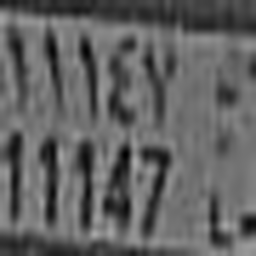
\includegraphics[width=0.8\linewidth]{../assets/gray.png}\\{\scriptsize image (spatial)}
    \end{center}\end{column}
    \begin{column}{0.5\textwidth}\begin{center}
      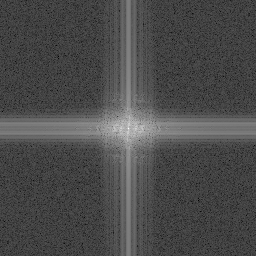
\includegraphics[width=0.8\linewidth]{../assets/spectrum.png}\\{\scriptsize magnitude spectrum (log)}
    \end{center}\end{column}
  \end{columns}
  \vspace{3pt}
  \begin{itemize}
    \item Centre = low frequencies (DC = average brightness). Edges = high frequencies.
    \item Bright lines/points reveal dominant orientations and repeating structure.
  \end{itemize}
\end{frame}

\begin{frame}{Reading the spectrum}
  \begin{itemize}
    \item The \term{centre} is the average; energy usually concentrates there (natural images are mostly low-freq).
    \item A strong \term{direction} in the image $\rightarrow$ a bright line \emph{perpendicular} to it in the spectrum.
    \item \term{Repeating patterns} (stripes, halftone) $\rightarrow$ isolated bright \term{peaks} off-centre.
  \end{itemize}
  \begin{infobox}
    We take the \code{log} of the magnitude to see anything — the DC term dwarfs everything else.
  \end{infobox}
\end{frame}

% ==================================================================
\section{Filtering in frequency}
% ==================================================================

\begin{frame}{Low-pass \& high-pass, done in frequency}
  \begin{columns}[T]
    \begin{column}{0.33\textwidth}\begin{center}
      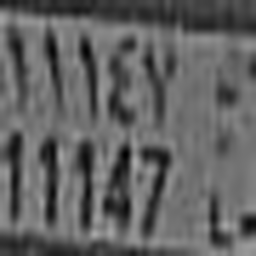
\includegraphics[width=\linewidth]{../assets/gray.png}\\{\scriptsize original}
    \end{center}\end{column}
    \begin{column}{0.33\textwidth}\begin{center}
      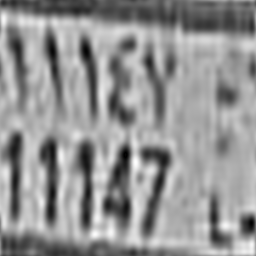
\includegraphics[width=\linewidth]{../assets/lowpass.png}\\{\scriptsize low-pass = blur}
    \end{center}\end{column}
    \begin{column}{0.33\textwidth}\begin{center}
      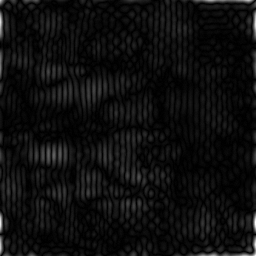
\includegraphics[width=\linewidth]{../assets/highpass.png}\\{\scriptsize high-pass = edges}
    \end{center}\end{column}
  \end{columns}
  \vspace{3pt}
  Keep the centre (low freq) $\rightarrow$ smoothing. Remove the centre (keep high) $\rightarrow$ edges.
  Same effects as Week 3, achieved by \emph{masking} the spectrum.
\end{frame}

\begin{frame}{Convolution theorem: why this matters}
  \begin{mathbox}
    Convolution in space $=$ multiplication in frequency: $f * h \;\longleftrightarrow\; F\cdot H$
  \end{mathbox}
  \begin{itemize}
    \item A big spatial convolution becomes a cheap element-wise multiply in frequency.
    \item For large kernels, FFT-based filtering is much faster ($O(N\log N)$ vs $O(N k^2)$).
    \item It's also \emph{why} the spatial and frequency views are two sides of one coin.
  \end{itemize}
\end{frame}

\begin{frame}{Ideal vs smooth filters (ringing)}
  \begin{itemize}
    \item An \term{ideal} sharp cutoff (a hard circle) causes \term{ringing} — ripples near edges.
    \item Smooth cutoffs (\term{Butterworth}, \term{Gaussian}) avoid ringing — the usual choice.
    \item Trade-off: sharper frequency selectivity $\leftrightarrow$ more spatial ringing.
  \end{itemize}
  \begin{badbox}
    A hard frequency mask can add wavy artifacts to a clean image. Prefer a gradual roll-off.
  \end{badbox}
\end{frame}

% ==================================================================
\section{Periodic noise}
% ==================================================================

\begin{frame}{Periodic noise: the killer app}
  \begin{columns}[T]
    \begin{column}{0.33\textwidth}\begin{center}
      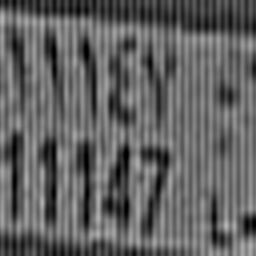
\includegraphics[width=\linewidth]{../assets/periodic_noisy.png}\\{\scriptsize striped noise}
    \end{center}\end{column}
    \begin{column}{0.33\textwidth}\begin{center}
      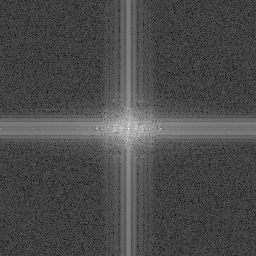
\includegraphics[width=\linewidth]{../assets/periodic_spectrum.png}\\{\scriptsize spectrum: 2 bright peaks}
    \end{center}\end{column}
    \begin{column}{0.33\textwidth}\begin{center}
      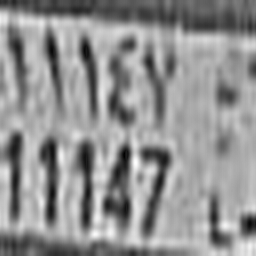
\includegraphics[width=\linewidth]{../assets/periodic_fixed.png}\\{\scriptsize after notch: clean}
    \end{center}\end{column}
  \end{columns}
  \vspace{3pt}
  \keyidea{Repeating stripes are a nightmare in the spatial domain — but two dots in frequency.
  Zero the dots (a \term{notch} filter), invert, done.}
\end{frame}

\begin{frame}{Notch filtering}
  \begin{itemize}
    \item A \term{notch} filter zeroes small regions of the spectrum (the noise peaks) and keeps the rest.
    \item Find the peaks (they're symmetric about the centre), mask them, inverse-transform.
    \item Perfect for scan lines, halftone patterns, sensor interference — real document artifacts.
  \end{itemize}
  \begin{goodbox}
    For DocScan: if a scanned form has a repeating background pattern, a notch filter removes it cleanly.
  \end{goodbox}
\end{frame}

\begin{frame}[fragile]{Fourier in code}
\begin{lstlisting}[language=Python]
F = np.fft.fftshift(np.fft.fft2(gray))     # to frequency, centre the DC
mag = 20*np.log(np.abs(F) + 1)             # log magnitude for display
# low-pass: keep a central disc
mask = make_circle_mask(gray.shape, r=30)
out = np.abs(np.fft.ifft2(np.fft.ifftshift(F * mask)))  # back to spatial
\end{lstlisting}
  \code{fft2} $\rightarrow$ mask $\rightarrow$ \code{ifft2}. The whole frequency workflow in three steps.
\end{frame}

% ==================================================================
\section{In-class exercise}
% ==================================================================

\begin{frame}{\faPen~In-class exercise (10 min)}
  \begin{infobox}[Predict the spectrum]
  \end{infobox}
  For each image, what does its magnitude spectrum look like?
  \begin{enumerate}
    \item A perfectly flat gray image.
    \item Vertical black-and-white stripes.
    \item A photo with lots of fine texture vs a smooth gradient.
    \item Where would you look in the spectrum to detect a repeating scan pattern?
  \end{enumerate}
\end{frame}

\begin{frame}{\faPen~Debrief}
  \begin{itemize}
    \item (1) Flat $\rightarrow$ a single point at the centre (only DC; no variation).
    \item (2) Vertical stripes $\rightarrow$ two symmetric points on the horizontal axis (one frequency).
    \item (3) Fine texture $\rightarrow$ lots of energy far from centre; smooth $\rightarrow$ energy hugging the centre.
    \item (4) Look for isolated bright peaks \emph{off-centre} — that's periodic structure.
  \end{itemize}
  \keyidea{The spectrum is a map of ``how much of each wave.'' Reading it becomes intuition with practice.}
\end{frame}

% ==================================================================
\section{Deep dive}
% ==================================================================

\begin{frame}{Amplitude vs phase}
  \begin{itemize}
    \item The DFT has \term{magnitude} (how much of each frequency) and \term{phase} (where it sits).
    \item Surprising fact: \term{phase} carries most of the \emph{structure} — swap two images' phases and you swap what you see.
    \item We visualize magnitude, but don't forget phase exists and matters.
  \end{itemize}
\end{frame}

\begin{frame}{FFT: why it's fast}
  \begin{itemize}
    \item A naive DFT is $O(N^2)$; the \term{Fast Fourier Transform} is $O(N\log N)$.
    \item This is what makes frequency-domain filtering practical on real images.
    \item Numpy/OpenCV give you the FFT; you just prepare the mask and invert.
  \end{itemize}
  \begin{mathbox}
    For a $1024^2$ image, FFT is $\sim$50{,}000$\times$ fewer operations than the naive sum.
  \end{mathbox}
\end{frame}

\begin{frame}{Other transforms (brief)}
  \begin{itemize}
    \item \term{DCT} (cosine transform): the heart of JPEG — compress by keeping low-frequency coefficients.
    \item \term{Wavelets}: multi-scale, localized in \emph{both} space and frequency — good for denoising \& compression.
    \item These are cousins of Fourier, each trading off localization vs frequency resolution.
  \end{itemize}
\end{frame}

\begin{frame}{When to use frequency vs spatial}
  \begin{itemize}
    \item \term{Frequency}: periodic noise, very large filters, analyzing texture/orientation.
    \item \term{Spatial}: local operations, edges, morphology, anything position-dependent.
    \item Most day-to-day work is spatial; frequency is the right tool for specific jobs.
  \end{itemize}
  \keyidea{Don't reach for the FFT by default — but when you see a repeating pattern, it's exactly the tool.}
\end{frame}

\begin{frame}{Aliasing, in the frequency view}
  \begin{itemize}
    \item Week 1's aliasing is clearest here: sampling replicates the spectrum; if it's too wide, copies \term{overlap}.
    \item Overlapping spectra = high frequencies folding into low ones = the moir\'e/jaggies you saw.
    \item Blur (low-pass) before downsampling narrows the spectrum so copies don't overlap — anti-aliasing.
  \end{itemize}
\end{frame}

\begin{frame}{Homomorphic filtering (brief)}
  \begin{itemize}
    \item Uneven lighting is low-frequency; reflectance (the content) is higher-frequency.
    \item Take the log, then high-pass slightly to suppress illumination and boost detail.
    \item Useful for a document photographed under a gradient of light — flattens the shading.
  \end{itemize}
  \begin{goodbox}
    Another DocScan trick: homomorphic filtering can even out lighting before thresholding.
  \end{goodbox}
\end{frame}

\begin{frame}{Frequency thinking $\rightarrow$ deep learning}
  \begin{itemize}
    \item CNNs learn spatial kernels, but the frequency view explains what they capture (edges = high-freq).
    \item Some modern architectures operate partly in frequency for efficiency.
    \item Understanding frequency deepens your intuition for what any filter — hand-made or learned — does.
  \end{itemize}
\end{frame}

% ==================================================================
\section{Wrap-up}
% ==================================================================

\begin{frame}{What you should now be able to do}
  \begin{itemize}
    \item Explain an image as a sum of waves; read a magnitude spectrum.
    \item Low/high-pass filter by masking the spectrum; know about ringing.
    \item Remove periodic noise with a notch filter (the killer application).
    \item Use the convolution theorem to reason about speed and equivalence.
  \end{itemize}
\end{frame}

\begin{frame}{This week's deliverable}
  \begin{alertblock}{Due before Week 7 (see \code{project/})}
    \begin{enumerate}
      \item Compute and display the magnitude spectrum of 3 real images; interpret each.
      \item Implement low-pass and high-pass by masking; compare to spatial blur/edges.
      \item Add periodic (stripe) noise; locate the peaks; remove it with a notch filter.
      \item Note: when is frequency-domain the right tool for a DocScan problem, and when not?
    \end{enumerate}
  \end{alertblock}
\end{frame}

\begin{frame}[standout]
  An image is a sum of waves.\\[4pt]
  \normalsize Some problems that are impossible in space are trivial in frequency.
\end{frame}

\end{document}
